\documentclass{beamer}

\usepackage[utf8]{inputenc}
\usepackage{hyperref}

\usetheme{Berkeley}
\beamertemplatenavigationsymbolsempty
\setbeamertemplate{headline}{}
 
\title{Importing data into FoodChain-Lab with All-in-one template}
\date{}
 
\begin{document}
\maketitle

\section{Tasks}
\begin{frame}
	\begin{itemize}
		\item In this tutorial we'll show you how to import delivery data to FoodChain-Lab via our All-in-one Excel template.
		\item All data will be entered in one file.
		\item The All-in-one template can be download from here: \url{https://github.com/SiLeBAT/BfROpenLabResources/raw/master/GitHubPages/templates/All_In_One_Template.xlsx}
	\end{itemize}
\end{frame}
 
\section{1}
\begin{frame}
	\begin{center}
  		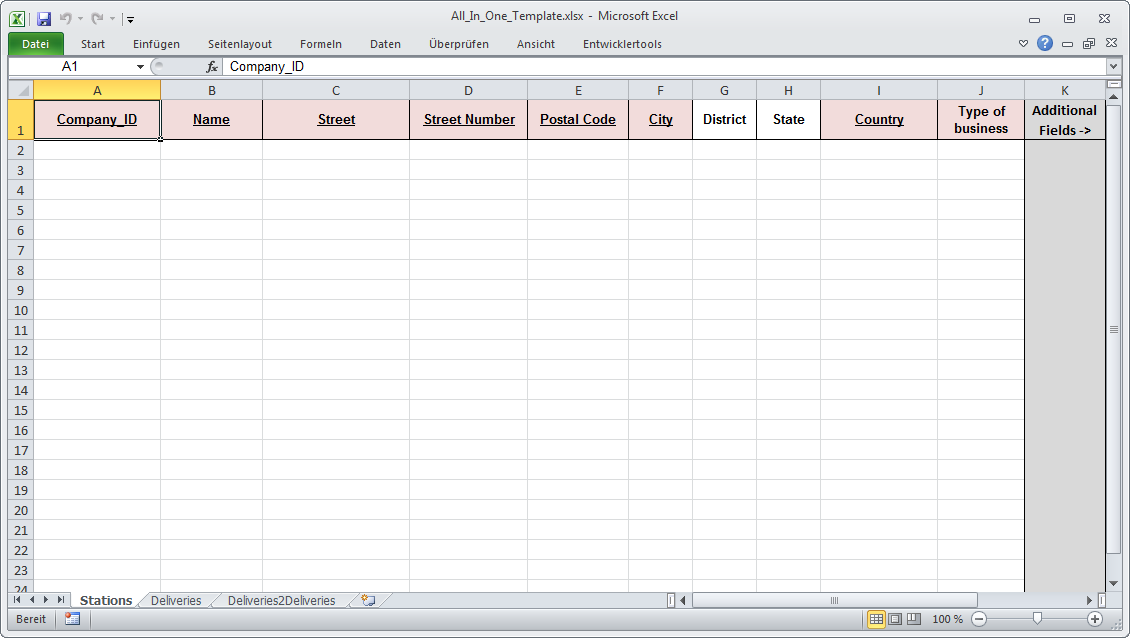
\includegraphics[height=0.5\textheight]{1.png}
	\end{center}
	\begin{itemize}
		\item Open \textbf{All\_In\_One\_Template.xlsx} and select the \textbf{Stations} sheet.
		\item Here you must enter all stations of the delivery network.
		\item The columns with the red header are predefined and some of them are mandatory.
		\item Next to \textbf{Additional Fields} you can specify your own columns, for which you would like to enter data.
	\end{itemize}
\end{frame}

\section{2}
\begin{frame}
	\begin{center}
  		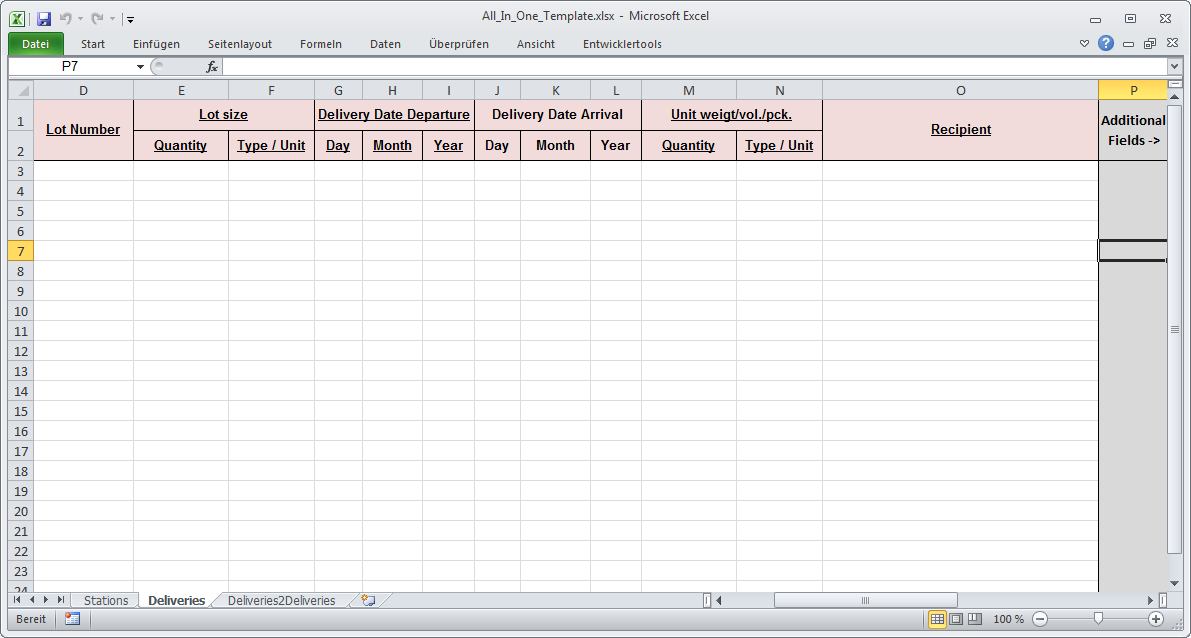
\includegraphics[height=0.6\textheight]{2.png}
	\end{center}
	\begin{itemize}
		\item Now select the \textbf{Deliveries} sheet.
		\item Here you must enter all deliveries between the stations defined in the previous sheet.
		\item
	\end{itemize}
\end{frame}

\section{3}
\begin{frame}
	\begin{center}
  		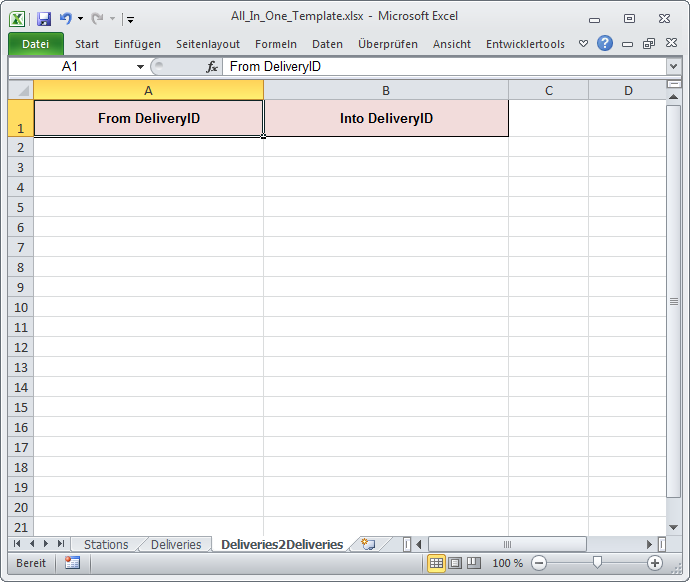
\includegraphics[height=0.6\textheight]{3.png}
	\end{center}
	\begin{itemize}
		\item
	\end{itemize}
\end{frame}

\section{4}
\begin{frame}
	\begin{center}
  		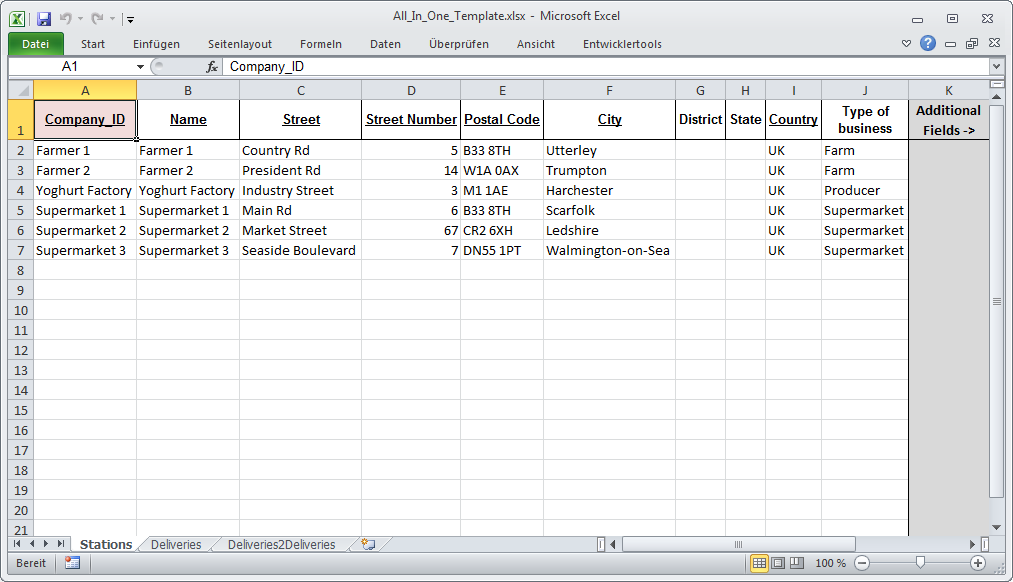
\includegraphics[height=0.6\textheight]{4.png}
	\end{center}
	\begin{itemize}
		\item
	\end{itemize}
\end{frame}

\section{5}
\begin{frame}
	\begin{center}
  		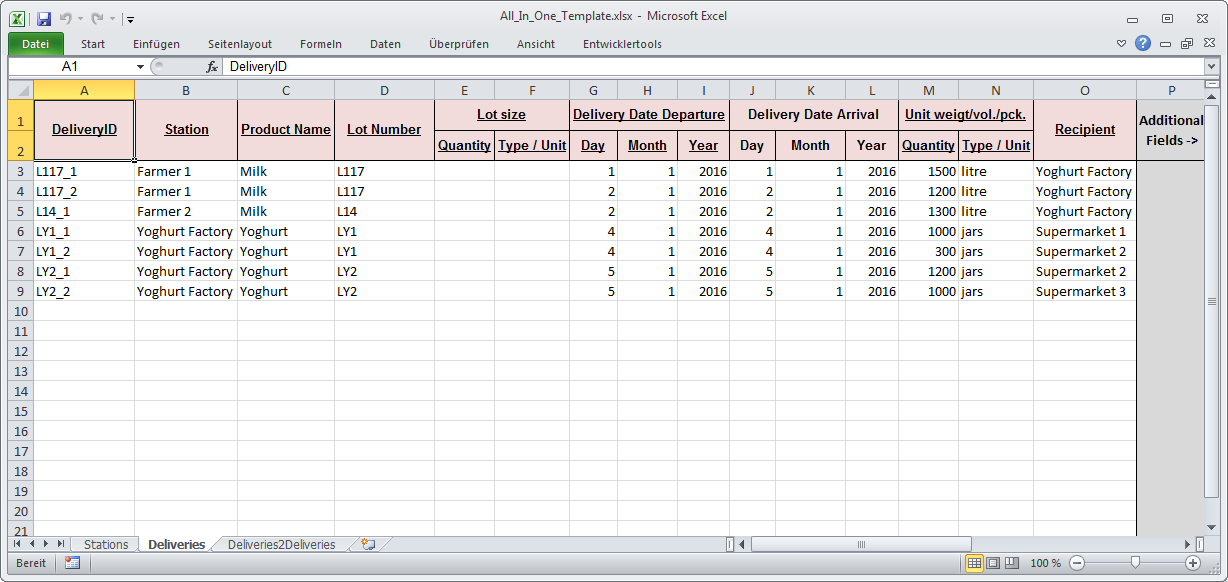
\includegraphics[height=0.6\textheight]{5.png}
	\end{center}
	\begin{itemize}
		\item
	\end{itemize}
\end{frame}

\section{6}
\begin{frame}
	\begin{center}
  		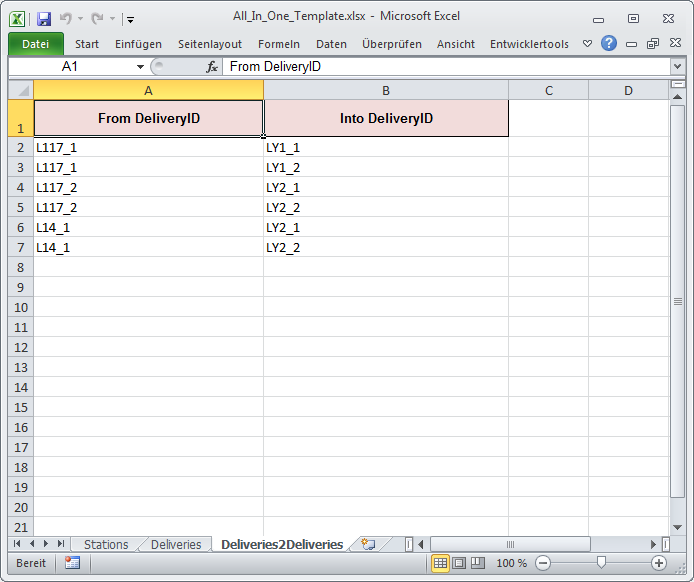
\includegraphics[height=0.6\textheight]{6.png}
	\end{center}
	\begin{itemize}
		\item
	\end{itemize}
\end{frame}

\end{document}